\documentclass[12pt]{article}
%\usepackage{geometry}                % See geometry.pdf to learn the layout options. There are lots.
                 % ... or a4paper or a5paper or ... 
%\geometry{landscape}                % Activate for for rotated page geometry
%\usepackage[parfill]{parskip}    % Activate to begin paragraphs with an empty line rather than an indent
\usepackage[top=1in, bottom=1in, left=1in, right=1in]{geometry}
\geometry{letterpaper}  
\usepackage{graphicx}
\usepackage{amssymb}
\usepackage{amsmath}
\usepackage{epstopdf}
\usepackage{subfigure}
\usepackage[numbers,sort]{natbib}
%\usepackage[LGR,T1]{fontenc} %% LGR encoding is needed for loading the package gfsneohellenic
%\usepackage[default]{gfsneohellenic}
\DeclareGraphicsRule{.tif}{png}{.png}{`convert #1 `dirname #1`/`basename #1 .tif`.png}

%\title{Forgetting}
%\author{Frank Wood\\Columbia University\\Department of Statistics}
%\date{\today}                                           % Activate to display a given date or no date

% !TEX root = talk.tex

\newcommand{\comment}[1]{}
%\newcommand{\comment}[1]{{\marginpar{\tiny {#1} }}}

\def\bigO{{\mathcal O}}
\def\balpha{\mbox{\boldmath $\alpha$}}
\def\bbeta{\mbox{\boldmath $\beta$}}
\def\beeta{\mbox{\boldmath $\eta$}}
\def\blambda{\mbox{\boldmath $\lambda$}}
\def\bmu{\mbox{\boldmath $\mu$}}
\def\bphi{\mbox{\boldmath $\phi$}}
\def\bpsi{\mbox{\boldmath $\psi$}}
\def\bsigma{\mbox{\boldmath $\sigma$}}
\def\btau{\mbox{\boldmath $\tau$}}
\def\btheta{\mbox{\boldmath $\theta$}}
\def\dbphi{\dot{\mbox{\boldmath $\phi$}}}
\def\dbtau{\dot{\mbox{\boldmath $\tau$}}}
\def\dbtheta{\dot{\mbox{\boldmath $\theta$}}}

%\newcommand{\nofootnotemark}{\let\@makefnmark\relax}
\newcommand{\bX}{\mathbf{X}}
\newcommand{\bY}{\mathbf{Y}}
\newcommand{\bW}{\mathbf{W}}
\newcommand{\bZ}{\mathbf{Z}}
\newcommand{\bH}{\mathbf{H}}
\newcommand{\bQ}{\mathbf{Q}}
\newcommand{\bA}{\mathbf{A}}
\newcommand{\bI}{\mathbf{I}}
\newcommand{\by}{\mathbf{y}}
\newcommand{\bz}{\mathbf{z}}
\newcommand{\bx}{\mathbf{x}}

\newcommand{\ith}{i^\mathrm{th}}
\def\A{{\bf A}}
\def\B{{\bf B}}
\def\C{{\bf C}}
\def\D{{\bf D}}
\def\F{{\bf F}}
\def\L{{\bf L}}
\def\M{{\bf M}}
\def\W{{\bf W}}
\def\I{{\bf I}}
\def\J{{\bf J}}
\def\R{{\bf R}}
\def\U{{\bf U}}
\def\V{{\bf V}}
\def\b{{\bf b}}
\def\c{{\bf c}}
\def\d{{\bf d}}
\def\r{{\bf r}}
\def\s{{\bf s}}
\def\t{{\bf t}}
\def\u{{\bf u}}
\def\v{{\bf v}}
\def\f{{\bf f}}
\def\x{{\bf x}}
\def\y{{\bf y}}
\def\w{{\bf w}}
\def\vo{{\bf o}}
\def\p{{\bf p}}
\def\O{{\bf 0}}
%\def\a{{\bf a}}


\def\vbpsi{\vec{\mbox{\boldmath $\psi$}}} 
\def\vpsi{\vec{\psi}} 
\def\vbphi{\vec{\mbox{\boldmath $\phi$}}} 
\def\vphi{\vec{\phi}} 
\def\vbtau{\vec{\mbox{\boldmath $\tau$}}} 
\def\vbtheta{\vec{\mbox{\boldmath $\theta$}}} 
\def\vD{\vec{D}}
\def\vf{\vec{\bf f}}
\def\vF{\vec{\bf F}}
\def\vI{\vec{\bf I}}
\def\vR{\vec{\bf R}}
\def\vv{\vec{v}}
\def\vV{\vec{\bf V}}

\def\pon{p_{\mathrm{on}}}
\def\poff{p_{\mathrm{off}}}

\def\tr{^{\text{T}}}

%%% Vector notation for sections 3 and 4
%%% Vector notation for sections 3 and 4
\def\mvec{\vec{m}}
\def\fvec{\vec{f}}
\def\appfvec{\vec{f}_k}
\def\avec{\vec{a}}
\def\bvec{\vec{b}}
\def\evec{\vec{e}}
\def\uvec{\vec{u}}
\def\xvec{\vec{x}}
\def\wvec{\vec{w}}
\def\gradvec{\vec{\nabla}}

\def\aM{\mbox{\bf a}_M}
\def\aS{\mbox{\bf a}_S}
\def\aO{\mbox{\bf a}_O}
\def\aL{\mbox{\bf a}_L}
\def\aP{\mbox{\bf a}_P}
\def\ai{\mbox{\bf a}_i}
\def\aj{\mbox{\bf a}_j}
\def\an{\mbox{\bf a}_n}
\def\a1{\mbox{\bf a}_1}
\def\a2{\mbox{\bf a}_2}
\def\a3{\mbox{\bf a}_3}
\def\a4{\mbox{\bf a}_4}

%\def\x{\mbox{\bf x\/}}
%\def\X{\mbox{\bf X}}
%\def\A{\mbox{\bf A}}
%\def\P{\mbox{\bf P}}
%\def\C{\mbox{\bf C}}
%\def\c{\mbox{\bf c}}
%\def\b{\mbox{\bf b}}
%\def\o{\mbox{\bf o}}
%\def\h{\mbox{\bf h}}
%\def\f{\mbox{\bf f}}
%\def\x{\mbox{\bf x}}
%\def\sx{\mbox{\scriptsize\bf x}}
%\def\z{\mbox{\bf z}}
%\def\l{\mbox{\bf l}}
%\def\m{\mbox{\bf m}}
%\def\bi{\mbox{\bf i}}
%\def\u{\mbox{\bf u}}
%\def\v{\mbox{\bf v}}
\def\a{\mbox{\bf a}}
%\def\p{\mbox{\bf p}}
%\def\r{\mbox{\bf r}}
%\def\d{\mbox{\bf d}}
%\def\Q{\mbox{\bf Q}}
%\def\s{\mbox{\bf s}}
%\def\st{\mbox{\scriptsize\bf t}}
%\def\ss{\mbox{\scriptsize\bf s}}
%\def\t{\mbox{\bf t}}
%\def\cR{{\cal R}}
%\def\calD{{\cal D}}
%\def\calS{{\cal S}}
%\def\g{\mbox{\bf g}}
%\def\e{\mbox{\bf e}}
%\def\flow{\{\mbox{\bf u}\}}
%\def\appearChange{iconic change}

\def\sigmae{\sigma}
\def\sigmam{\sigma}

\newcommand{\eg}{e.\thinspace{}g.,\@\xspace}
\newcommand{\egn}{e.\thinspace{}g.\@\xspace}
\newcommand{\cf}{cf.\@\xspace}
\newcommand{\ie}{i.\thinspace{}e.,\@\xspace}
\newcommand{\ien}{i.\thinspace{}e.\@\xspace}
\newcommand{\iid}{i.\thinspace{}i.\thinspace{}d.\@\xspace}


%\newcommand{\comment}[1]{}
\newcommand{\ponedec}{\mathcal{P}^\downarrow_1}
\newcommand{\pone}{\mathcal{P}_1}
\newcommand{\rank}[1]{\mathrm{RANK}\left[#1\right]}
%\newcommand{\E}[1]{\mathrm{E}\left[#1\right]}
%\newcommand{\PY}{\mathcal{PY}}
%\newcommand{\DP}{\mathcal{DP}}
%\newcommand{\iid}{iid.}
\newcommand{\drawiid}{\stackrel{\text{iid}}{\sim}}
\newcommand{\vect}[1]{\mathbf{#1}}
\newcommand{\indicator}[1]{\text{I}\left[ #1 \right]}
\newcommand{\pdcoag}{PD(d_1,0)-\text{COAG}}
%\newcommand{\todo}{\textbf{*TODO*}}
\newcommand{\igram}{\text{$\infty$-gram}}
\newcommand{\Prob}{\text{P}}

\def\mm{sequence memoizer }
\def\MM{SM }

\def\pibf{{\boldsymbol{\pi}}}
\def\kapbf{\boldsymbol{\kappa}}
\def\taubf{\boldsymbol{\tau}}
\def\thebf{\boldsymbol{\theta}}
\def\rhobf{\boldsymbol{\rho}}
\def\phibf{\boldsymbol{\phi}}
\def\pbf{\mathbf{p}}
\def\qbf{\mathbf{q}}
\def\sbf{\mathbf{s}}
\def\tbf{\mathbf{t}}
\def\ybf{\mathbf{y}}
\def\ubf{\mathbf{u}}
\def\Ave{\mathbb{E}}

\def\wbf{\mathbf{w}}
\def\xbf{\mathbf{x}}
\def\rbf{\mathbf{r}}
\def\tbf{\mathbf{t}}
\def\kbf{\mathbf{k}}
\def\Xbf{\mathbf{X}}
\def\0bf{\mathbf{0}}
\def\Ibf{\mathbf{I}}
\def\phibf{\mathbf{\phi}}
\def\Phibf{\mathbf{\Phi}}
\def\disteq{{\stackrel{D}{=}}}
\def\GG{\mathcal{G}}
\def\G{G}
\def\U{U}

\def\phiv{\varphi}
\def\phivbf{\boldsymbol{\varphi}}

\def\Ocal{\mathcal{O}}
\DeclareMathOperator*{\Var}{Var}

\DeclareMathOperator*{\Bet}{Beta}
\DeclareMathOperator{\coag}{COAG}
\DeclareMathOperator{\frag}{FRAG}
\DeclareMathOperator*{\rnk}{RANK}
\DeclareMathOperator*{\gem}{GEM}
\DeclareMathOperator*{\pd}{PD}
\DeclareMathOperator*{\py}{PY}
\DeclareMathOperator*{\DP}{DP}
\DeclareMathOperator*{\PY}{PY}
\DeclareMathOperator*{\gd}{GDir}
\DeclareMathOperator*{\Dir}{Dir}
\DeclareMathOperator*{\CRP}{CRP}
\DeclareMathOperator*{\argmax}{argmax}

\def\GG{\mathcal{G}}
\def\data{\mathbf{x}}
\def\EE{\mathbb{E}}
\def\disc{d}
\newcommand{\delete}[1]{} %\textcolor{red}{#1}
\newcommand{\rewrite}[1]{#1}%{\textcolor{blue}{#1}} %
\newcommand{\lambdabf}{\boldsymbol{\lambda}}
\newcommand{\vbf}{\mathbf{v}}
\newcommand{\Psmooth}{\Prob_\text{smooth}}
%\newcommand{\parent}{\pi}
\newcommand{\suffix}{\sigma}
\newcommand{\UHPYP}{SM}
\newcommand{\PLUMP}{PLUMP}
\newcommand{\Oh}{\mathcal{O}}
\newcommand{\tree}{\mathcal{T}}
\newcommand{\cct}{\hat{\mathcal{T}}}
\newcommand{\cctx}{\cct(\data)}
\newcommand{\Gu}{G_{\ubf}}
\newcommand{\GuSet}{\{G_{\ubf}\}_{\ubf \in \Sigma^*}}
\newcommand{\E}{\mathrm{E}}
\newcommand{\UpdatePath}{\text{\textsc{UpdatePath}}}
\newcommand{\Path}{\ensuremath{(\ubf_0,\ldots,\ubf_P)}}
\newcommand{\PathProbability}{\text{\textsc{PathProbability}}}
\newcommand{\TT}{\mathcal{T}}
\newcommand{\ral}[1]{\stackrel{\mathtt{#1}}{\rightarrow}}
\def\parent{{\sigma(\mathbf{u})}}

%\def\newblock{\hskip .11em plus .33em minus .07em}


% \newcommand{\cusk}{c_{\ubf s k}}
% \newcommand{\cus}{c_{\ubf s \cdot}}
% \newcommand{\cu}{c_{\ubf \cdot \cdot}}
% \newcommand{\tus}{t_{\ubf s}}
% \newcommand{\tu}{t_{\ubf \cdot}}
\newcommand{\cusk}{c_{\ubf s k}}
\newcommand{\cus}{c_{\ubf s}}
\newcommand{\cu}{c_{\ubf \cdot}}
\newcommand{\tus}{t_{\ubf s}}
\newcommand{\tu}{t_{\ubf \cdot}}
\newcommand{\cset}{\{\cusk\}_{s\in \Sigma,k \in \{1,\ldots,t_{\ubf s}\}}}
\newcommand{\tset}{\{\tus\}_{s\in \Sigma}}
\newcommand{\bydef}{\equiv}
\newcommand{\state}{\mathcal{S}_{\xbf}}
\newcommand{\statei}{\mathcal{S}_{\xbf_{1:i}}}
%\newcommand{\emptystring}{\varepsilon}
\newcommand{\gcount}{\hat{c}}
\newcommand{\escape}{\mathtt{esc}}
\def\prob{G}


\newcommand{\todo}[1]{\begin{center}\textbf{TODO: } #1 \end{center}}
\newcommand{\figref}[1]{\figurename~\ref{#1}}
\newcommand{\predictive}{\Prob(x_i|\xbf_{1:i-1})}
\newcommand{\ywcomment}[1]{\textbf{#1}}
\newcommand{\jgcomment}[1]{ { \textcolor{red}{#1} } }

\newcommand{\secref}[1]{Section \ref{#1}}

\def\context{\mathbf{u}}

%%% Local Variables: 
%%% mode: latex
%%% TeX-master: "paper"
%%% End: 


\begin{document}
%\maketitle
\begin{center} \bf \Large Hierarchical Bayesian Models for Artificial Intelligence \end{center}
%
%A Step Towards Fully-Unsupervised, Life-Long, Incremental Learning

%Exploring the marriage of massive data to unsupervised, deep hierarchical nonparametric Bayesian learners.
%\section{Principle Investigators}
%
\begin{center}
\begin{tabular}{llll}
{\bf PI }& Frank Wood, Ph.D. &{\bf Position }& Assistant Professor\\
{\bf Address} & Room 1005 SSW, MC 4690 & {\bf University} & Columbia University \\
&1255 Amsterdam Avenue & {\bf Department }& Statistics \\
&New York, NY 10027 \\
 {\bf Phone} & 212.851.2132& {\bf Fax} & 212.851.2164 \\
 {\bf Website} &{http://www.stat.columbia.edu/$\sim$fwood}\\
 %& \multicolumn{2}{l}{http://www.stat.columbia.edu/$\sim$madigan}
\end{tabular}
\end{center}

%\subsection{Abstract}
\begin{quote}
\begin{center}
\bf \scshape Abstract
\end{center}
%\scshape
We propose to test the hypothesis that hierarchical Bayesian nonparametric (BNP) models can be used to learn compact world representations suitable for efficient artificial intelligence (AI) search and planning.  

%\vspace{-.05cm}
{\bf Keywords :} hierarchical models, Bayesian nonparametrics

\vspace{-.1cm}
{\bf Research Areas :} machine learning, unsupervised probabilistic modeling
\end{quote}
%\subsection{Goals}

%\noindent {\bf Goal} 
%\begin{itemize}
%\item Artificial intelligence
%\end{itemize}

%\noindent {\bf Expected Outcome} 
%\begin{itemize}
%\item Failure
%\end{itemize}
\newpage
%\noindent{\bf \large Big Picture}
%\vspace{.1cm}

%\noindent The field of artificial intelligence (AI) has been unfairly stigmatized by continuing disappointment about the perceived lack of progress, particularly in comparison to promises made.  The persistence of this slight is somewhat curious, particularly since we now know much more about the true difficulty of the challenge and how difficult it would have been to deliver on early promises like ``machines will be capable, within twenty years, of doing any work that a man can do'' [Simon, 1965].  Now we know that ``the hard problems are easy and the easy problems are hard. The mental abilities of a four-year-old that we take for granted -- recognizing a face, lifting a pencil, walking across a room, answering a question -- in fact solve some of the hardest engineering problems ever conceived,''  [Pinker, 2007].

%AI is high-risk, high-return research -- precisely the kind of research conservative federal funding agencies strain to support, but also precisely the kind of research that can lead to both incredible, direct improvements to the well-being of all people and indirect, but potentially even greater impact on the way knowledge is discovered.


%Most machine learning researchers avoid even stating the AI goal and retreat to the incremental and cautious pursuit of theoretical and empirical performance improvements to well studied engineering problems such as binary and multi-class classification.  The end-product of this kind of work is valuable but extremely unlikely to ``rock the world'' as AI would. Dream for a second about the economic, social, and political ramifications of the achievement of human-level AI:  even quick, back-of-the-envelope, rational consideration of just the economic net-present-value of human-level AI makes its direct pursuit imperative.   

%AI has always been and always will remain my goal.  I know very well how hard the problem is, but am willing to invest my life trying to succeed anyway.  I maintain that research that contributes meaningfully to the plausibility of AI should be funded.   
%This is because the achievement of AI would be a profound return on investment.  AI research is not like research to increase the efficiency of solar panels by 15\%, a directly, economically measurable contribution.  AI would utterly transform the world for the better; socially, economically, and politically.  

%With respect to the more practical issue of pursuing funding, a famous and well-funded Carnegie Mellon machine learning\footnote{The field even picked a new name!} professor told me recently ``if you want to get funding, don't dare mention artificial intelligence.  Mention some other application then work on whatever AI related thing you really want to.''  To this I call "bullshit!" 

%More directly;  even completely ignoring the economic value of replacing human labor, the pursuit of {\em all} research -- the search to cure AIDS, cancer, and other diseases; the quest to understand the universe and our place in it; etc --  {\em all} would be dramatically impacted and streamlined by the ``tool'' of artificial intelligence.  It can be argued along these lines that artificial intelligence funding levels should be at a minimum a non-trivial fraction of the total budget spent to develop new tools for experimental science.

\vspace{.4cm}
\noindent{\bf Artificial Intelligence}
\vspace{.1cm}

\noindent Artificial intelligence is arguably best posed as a search problem \cite{Russell2002}.  Given a goal (reproductive success, crossing a street, winning a game of chess or poker), achievement of that goal can be phrased as the problem of searching through a space of possible future worlds to find the action that optimizes the probability or amount of future reward.  %Games are a particularly easy but somewhat deceptive case study for formalizing this problem.  
%Call the chess board and the current positions of all of the pieces on the board the ``state'' of the ``world.''   Now, let's say that you receive a ``reward'' at the end of every game you play: 1 if you checkmate your opponent,  -1 for the other way around, and 0 for everything else.  The reward yielded by each game-ending state can be computed simply by observing the state of the board.  Either the board is in checkmate for you or against you, or it's in some other state from before you and your partner agreed to a draw.  Easy.  What's much, much harder is figuring out what action to take when the world is in some particular intermediate state.  Often there are many moves that could be made, each leading towards a potentially different set of outcomes and corresponding rewards.  The optimal way to choose what to do next is to choose the action that maximizes the probability (or amount) of positive reward.   The problem is that to calculate this quantity, one must simulate all possible next moves for you and your opponent to all possible conclusions of the game.  This, of course, is a huge ``space'' of worlds to consider. 
% If there are on average 10 possible moves you could take, 10 possible moves your partner could take in return, and it takes on average 10 possible moves to reach the end of the game from your current state, then the number of possible ending states that must be considered in order to make a single move is (naively) $10^{20}$ (a {\em lot}).
%If you could compute all possible outcomes somehow, you would simply choose the action that maximizes the probability of future positive reward.  
This setup is very general; almost any planning problem can be posed and solved using this formalism.  Unfortunately, for most interesting problems the search space typically gets very big and therefore becomes computationally intractable.
%latent feature spaces
Pruning the search space is the only way render the search problem tractable in general.  Learning models of the world that explain high-dimensional observations in terms of simpler, unobserved, but sufficiently explanatory latent states is one way to do this.  How to do this is arguably the biggest problem that must be solved in order to develop AI.   %When thinking about how the world is perceived by a computer it is very important to put aside human intuitions about what data looks like.  To a computer the world is merely a sequence of changing bits.    Human plans are formed by searching through low dimensional, causal descriptions of wor and not through a world of individual pixels and video segments.  Such latent world descriptions can be thought of as generating the observations; the question is how to discover such low-dimensionality latent descriptions of observed worlds and which one is right?
%Consider, for example, the problem of learning how to perform a straight-line crossing of a busy street from fixed-camera visual input.  
%The dimension of the raw observations of this world, the naive space which must be searched to form a rewarding crossing plan, is of dimension proportional to the length of time it takes to cross the street times the resolution of the video.  As always, it is important to put aside human intuitions about what this data looks like.  To a computer this world is merely a sequence of changing video frames composed of pixels, themselves simply bunches of changing bits.  This is not dissimilar to the data that impinges upon your retina when you perform this task yourself.  Your percept of such scenes, however, provides strong evidence that you use a compressed, latent representation of the world to both learn and form your plans.   Your percept of a street crossing scene is one of a  world and its evolution featuring latent objects such as background elements like the street and sky; foreground objects and their characteristics like automobiles, their speeds, direction, and (usually) intent; and more.  
%This percept is invariant in many ways.  It does not change even though your perspective and the data impinging on your retina correspondingly changes as you cross the street.  Your percept of a car is constant despite the fact that the car moves and may change in visual characteristic significantly.  
%A plan must be found by simulating and searching through a learned model of the key features of the world like the positions and velocities of the cars on the street, not by searching through the high-dimensional state space defined by the changing values of pixels in video frames.  
%The question is how to automatically learn the right simple latent descriptions of complex observed worlds.  
This is the over-arching theme of my work.

%Consider the following question answering example.  A question is a sequence of characters and thus correspondingly a sequence of bits.  An answer is the same.  Consider the question, ``What will happen to a basketball dropped from the top of the Empire State building?''  In this case what are the states of the world?  If the states of the world are question answer string pairs, then the only response that one could hope to give to this question is the answer given in previous situations.

%s; collision avoidance and question answering.   An example of collision avoidance is learning how to navigate through arbitrary rooms with doors on either end with single obstacle sitting in the middle of the room (for instance a table) from visual input.  The search for an optimal path is tractable, even easy, if the visual representation of the world is preprocessed into on in which the relative position of obstructing objects are represented by a three dimensional bounding boxes, the extent of the room and the location of the doors are represented as boxes in three dimensions, and the position and extent of the robot are also specified by a small list of numbers indicating positions in some Cartesian reference frame.  Then both planning and learning become easy.  


% from relatively little training data, and prioritizing search over sequences of ``most likely'' next states both can significantly prune the dimensionality of the search space.

%Figuring out computationally practical ways choose actions, even in ``simple'' world such as the one defined by the rules of chess, requires one to consider ways to ``prune'' the search space.  One way to do this is to prioritize your search according to predictions made about what your opponent will do.  If you knew exactly what your opponent would do

%There are, thankfully, ways to render the choice of future action more computationally tractable; 1) reuse computation, 2) choose actions sub-optimally 3) discover representations of the world that are ``lower dimensional.''  ``Dynamic programming'' is the name given to standard techniques for reusing computation.  An example of this is as follows: if one computes the reward for all game ending states then computing the distribution over rewards for all game states that are one move away from an end state is easy.  Continuing in this ``bottom up'' fashion ensures no obviously wasted computation.  Behaving sub-optimally is easy -- one can either simply not compute all possible outcomes for each possible next move, use heuristics to compute the ``goodness'' of states at some arbitrary depth of search, or simply not consider certain moves.
%It is the last approach to making search more computationally tractable that I focus on.  A trivial kind of lower dimensional world representation is one that recognizes that many states of the world are equivalent, usually due to symmetries of various kinds (in our example, the bishops, knights, and rooks are indistinguishable from each other and need not be individually labeled, almost all game states with only two kings remaining are equivalent, etc.).  More sophisticated methods of learning about latent states of the world {\em can} lead to action choice that is near optimal with significantly less computational burden.

%One can visualize the space of game plays as a tree rooted at the board in its starting configuration and then branching to all states reachable by a single move.  Clearly because there is redundancy and symmetry in the pieces it is possible to arrive at the same state through different sequences of moves.  This can collapse the tree substantially.

%My work focuses on discovering representations of worlds that are ``low dimensional'' and then predicting things given that representation.  
%Imagine, though, having a model that could predict what move your opponent would make in response to your own, or, given the current state and your next move, the amount of award that would accrue on average if you were to take that move.  It might be possible, in many cases, to construct such a model without resorting to simulating all possible futures.  Improvements to predictive models of these kinds could be used to improve the performance of actors with respect to the amount of reward they accrue.

\vspace{.1cm}
\noindent{\bf Modeling}
\vspace{.1cm}

\noindent Probabilistic models are a mathematical framework for describing complex observations as the noise-corrupted output of simpler, often stochastic, latent mechanisms \cite{Bishop2006}.  The learned latent mechanism can be used for efficient AI planning and search.
%General purpose probabilistic modeling is still far from solved.  Take the inverse problem: given an arbitrary generative probabilistic model and a set of observations, how does one efficiently invert the model to figure out which settings of the latent states in the model were responsible for generating the observations?  Or the model selection problem: given a sequence of observations, how does one determine which latent mechanism is best?  Or the rule learning problem; given a setting of the latent states of the world, which rules best explain the evolution of the latent states?  I work on all of these problems.

I focus on learning models that satisfy an additional set of natural life-long learning requirements: models that are representable in constant space, incrementally updatable in constant time, and automatically adaptable to changes in the underlying world dynamics.  My focus thus-far has been on models that 
 fall at the bottom of a hierarchy of classical model complexity, but that actually are of infinite complexity; the simplest of which is an infinite Markov model called the sequence memoizer (SM) \cite{Wood2009}.  A Markov model describes the world as a deterministically transitioning state machine that generates noisy outputs from a known set of states.  The classical complexity and expressivity of a Markov model is a function of its number of states.  The SM has infinite state cardinality and therefore unbounded complexity, yet satisfies the life-long learning requirements \cite{Gasthaus2010,Bartlett2010,Bartlett2011}.  The SM achieves good performance because of hierarchical sharing of statistical strength between related states.
%Newtonian mechanics are the transition rules for a Markov model of the world whose states are the positions and momenta of all particles.   
%The street crossing problem can be posed and the planning problem solved using a Markov model of a world whose states are the measured positions and velocities of cars.  %Given the state of the world, simulating the evolution of the world for purposes of search is straightforward because of determinism but potentially problematic because such a model is a ``fully observed'' model and can't account for unobserved, latent states of the world.   

While Markov models like the SM are often very good models, they would seem to be representationally inefficient as the states in the model must be indexed by all observed features of the world.  %In a Markov model for a street crossing task, including traffic light state would be prudent but corresponds to a multiplicative expansion in the number of states.  
This state explosion is in conflict with AI model desiderata.  
The simplest kind of model that can counter this multiplicative state expansion is one that still transitions deterministically from state to state, but where these ``states'' are abstract, implicit to the model, and no longer in one-to-one correspondence with states of the world.   We have defined such a model called the probabilistic deterministic infinite automata, PDIA \cite{Pfau2010} that, like the the SM, also has an infinite state cardinality but, unlike the SM, is biased towards state reuse.  State reuse results in an overall simpler latent mechanism.  Unfortunately, hierarchical sharing of statistical strength is more difficult in the PDIA because the states in such a model lose their explicit correspondence with states in the world and it is unclear how such hierarchical sharing should be arranged.
%Imagine a model for the traffic light example in which a duplication of the original Markov states is learned, one each for the red and green light.  The inverse problem then becomes one of both inferring both where the cars are in the world while simultaneously inferring the unobserved state of the light.  

Others have worked on ``more complex'' models, also reposed on infinite state spaces, that allow for non-deterministic transitions between states \cite{Beal2002}, non-deterministic transitions with side memory \cite{Johnson2007}, and so on and so forth.  The classical analogs of these models are given different names by different scientific communities.  Computer scientists refer to these models as recognizers of formal languages in the Chomsky hierarchy \cite{Hopcroft1979}.   Statisticians generally refer to them by the name of the corresponding generative model: Markov model, finite state automata, hidden Markov model, probabilistic context free grammar, etc.  As a rule, in terms of classical complexity and expressivity, as one ascends this hierarchy the machines become more expensive to simulate, but more efficiently expressive on a per state basis.   In our experiments with this spectrum of infinitely complex models we have noticed a profoundly perplexing pattern.  For fixed-size data, the more complex (in the classical sense) models typically perform worse in general on real tasks.  There are many reasons why this could be so (broken inference, dominance of a misspecified prior, relative importance of state reuse vs.~hierarchical sharing, etc), but figuring out why this is so (when it should not be) is an important question we intend to address in this work.

The spectrum of models reposed on infinite state spaces are all hierarchical ``Bayesian nonparametric'' (BNP) models (the SM and PDIA form the bottom two rungs).  
%BNP models are characterized by infinite state cardinality and therefore unbounded expressivity). BNP models avoid within-family model selection problems, but complicate between-family model selection because they are not distinguishable in terms of classical complexity.  
BNP models can, in general, be made to conform to the AI modeling desiderata.  They have uniformly exhibited excellent empirical performance on a wide variety of tasks, are endowed with the attractive properties of nonparametric estimators, and typically (via exchangeability properties) can be estimated efficiently and incrementally from streaming data.  A variety of constant memory approximations to BNP models have been developed that also perform well.  All of this suggests that BNP models should perform well as the models in which AI search and planning are performed.  Whether this is true remains mostly unknown.  This is the main hypothesis that we aim to test.

\vspace{.1cm}
\noindent{\bf Summary}
\vspace{.1cm}

\noindent AI is a grand challenge.  Solving AI requires developing models that can represent the state of the world in a task specific way that generalizes well using simple and easy to simulate latent mechanisms.  Hierarchical BNP models exhibit many of the required characteristics, some of which have been highlighted here, more of which exist.  While BNP models are certainly not the only such models in the mix (deep belief nets, etc.), their utility for AI search and planning remains significantly under-explored.  Progress in BNP modeling has cross-cutting benefits; progress in BNP modeling for AI has the potential to produce very significant societal benefits.
%\begin{description}
%\item[Combining Search and Learning] It is an open question as to whether or not combining unsupervised learning with AI planning and search will result in different models being learned.  There is reason to suspect that the latent states learned in latent variable models might be improved by introducing task and reward-search-specific bias.  If so, this could lead to fundamental improvements to both unsupervised learning and to AI search and planning.
%\item[Explaining The Expressivity Conundrum]  In our experience, BNP models whose finite-dimensional counterparts increase in classical complexity often perform worse in terms of generalization performance.  This experience warrants significant investigation because it suggests that either inference is broken, there exists a rate of convergence issue whereby the the more ``complex'' models converge much too slowly, or the more complex priors bias significantly towards unnatural models.  We will investigate this conundrum and 
%\item[Finding Nature's Bias]  We have found that hierarchical sharing of statistical strength that encodes a ``recency matters'' assumption dominates all in terms of on the ground performance.
%\end{description}


%Every adult knows that humans are non-optimal participants in the game of life
%\footnote{See my own reproductive success.}.  
%We all somehow unconsciously learn and use ``low dimensional'' models of the world to guide our search for the best action to take given the state of the world.  For instance, we are able to infer the presence and features of objects in our environment from streaming visual observations, a massive dimensionality reduction from the space of pixels (or photon counts on photo-receptors) to attributes like extent, color, and location of a typically small number of objects.  Evidence of the kind of salient and meaningful low dimensional representations of the world we construct abound in our use of language to describe visual scenes, for instance: "there's a table in the middle of the room." This almost magically terse representation of a potentially complex visual scene is compressed (with loss) to an amazing degree but still manages to convey a surprisingly large amount of information about the original scene. 

%Linking this back to planning, in order for p
%So, for AI planning even to be remotely plausible, we must figure out how to learn representations the latent, causal world significantly compressed representation.  
%Unsupervised learning of predictive models of arbitrary worlds is, in the most general sense, the subject of my work.  Learning latent, low-dimensional representations of the world

%Discovering representations of worlds that are ``low dimensional'' and then predicting subsequent states of the world given that representation is the subject of my work.   
%To concretely link my own work on incremental predictive inference to the chess example above we need some additional terminology: let's call the states of the world in the example above ``words'' in some ``vocabulary.''
%  Given the number of positions pieces can take on a chessboard, the number of ``words'' in this ``vocabulary'' is tremendous.  Never-the-less, the problem of predicting what your opponent will do (for instance), given the sequence of moves up to that point in the game, can be phrased as a problem of predicting what the next word will be given a sequence of words observed up to that point.  If you think of the world as including your opponent then clearly a predictive model will tell you what state the world (word/positions of pieces) is likely to take in response to your move.  Building models of this nature is a very general pursuit.  Learning the parameters of such models in an efficient way that conforms to the computational constraints imposed by AI is challenging. 
  
%Consider this problem at its full level of abstraction.  Let $\x = x_1, x_2, ..., x_T$ be an observed sequence of words where each $x_t$ comes from some alphabet $\Sigma$.  Our goal is to be able to make predictions about what comes next after some ``context'' $\context \in \Sigma^+$, that is, after a sequence of words drawn from 
 
%Generative models often embed observations into rich, hierarchical, latent feature spaces.  A beautiful result of this is that we can express each observation as being "generated" by some mechanism indexed by some parameter vector.  Here the parameter vector is the latent feature representation.  Being a vector space, closeness between these vectors provides evidence that inference should be generalized between observations either sharing features/parameters or by shared between observations that are "close" in some metric sense.

%A suggestion/hint from Josh was that we need {\em programs} in order to be able to express rich enough generative procedures to solve the real problems of "learning/thought"  Unfortunately, a priori it is not obvious how to think of or treat "programs" as latent feature vectors.  In particular, computing a distance between programs can't be done in the metric sense.  In order to compute a distance between programs requires us to be able to generate programs.  This, for me, finally clarifies what it means to sit at some level on the Chomsky hierarchy.  The kinds of interactions between "features/objects" in a scene/context are constrained by the richness of the generative language.  We can't hope to build an AI that understands recursion without having a generative mechanism that supports it.  We can't hope to understand complex causal interactions between elements in a scene/context/observation without having a generative mechanism that itself can generate such interactions
 
\comment{  
Traditional parametric statistical tools and methods are designed to allow
inference about a population from a small sample.
While this parametric style of inference will always have a place, it is now the
case that one often has access to so much data that parametric models
themselves are sometimes not even necessary.  In other words, for some problems one can do strict nonparametric inference; i.e.~one can query
the data directly.  While such a nonparametric approach has attractive characteristics and  for some problems is feasible to consider, particularly given Google-scale data, we suggest that there are stochastic processes of sufficient complexity (e.g.~natural language generators) that strictly nonparametric approaches to estimation and inference (e.g.~non-smoothed $n$-gram language models) are bound to fail.  To attack these kinds of problems, we advocate and actively pursue computationally practical ways to estimate and perform inference in Bayesian nonparametric (BNP) models.   BNP models are nonparametric in nature, which gives them inferential capacity that can be understood to grow as a function of the amount of training data. Contrast this to parametric models in which inference is limited to inference through and about a finite set of parameters.   In parametric models as the amount of data grows, posterior uncertainty about the value of the parameters will vanish given sufficient data, rendering the inclusion of additional data irrelevant.  This is not true for BNP models, making them ideal for inference in the modern regime of continually growing data.  BNP models are are also Bayesian in nature which allows for hierarchical Bayesian-style regularization and incremental Bayesian-style inference and estimation.  For small scale data on the order of millions of observations, BNP natural language models and lossless compressors we have recently been shown to exhibit excellent empirical characteristics \citep{Teh2006a,Wood2009,Gasthaus2010}.  Unfortunately BNP models in general have been saddled with an unfortunate stigma, namely that they are as a class uniformly computationally complex. We suspect that this stigma is at least partially responsible for holding back wide adoption of BNP methods.   The work outlined in this proposal aims to chip away at this stigma by providing concrete evidence that at least one member of this class of BNP models scales well.

\vspace{.1cm}
\noindent{\bf \large Scaling the Sequence Memoizer}
\vspace{.1cm}

In recent work we established a rather surprising result: for non-antagonistically generated discrete sequence data (natural language token sequences, bytes, bits, etc.), we found that it was possible to estimate  the SM in the same asymptotic space and time as is required to estimate a smoothing $5$-gram model \citep{Wood2009} (\figref{fig1a}).  One way to understand the SM is as a Bayesian smoothing $n$-gram model in the limit of $n$ taken to infinity.  This means that the SM is capable of modeling long-range dependencies in discrete sequence data as opposed to finite-order Markov models which cannot.  What is more, in related work, we uncovered empirical evidence that supports Shannon's assertion \citep{Shannon1951} that long range dependencies in written language do exist and are significant up to and potentially extend beyond hundreds of characters \cite{Gasthaus2010} (related evidence for this can also be seen in \figref{fig1b}).  
\begin{figure}[htbp]
\begin{center}
\subfigure[]{
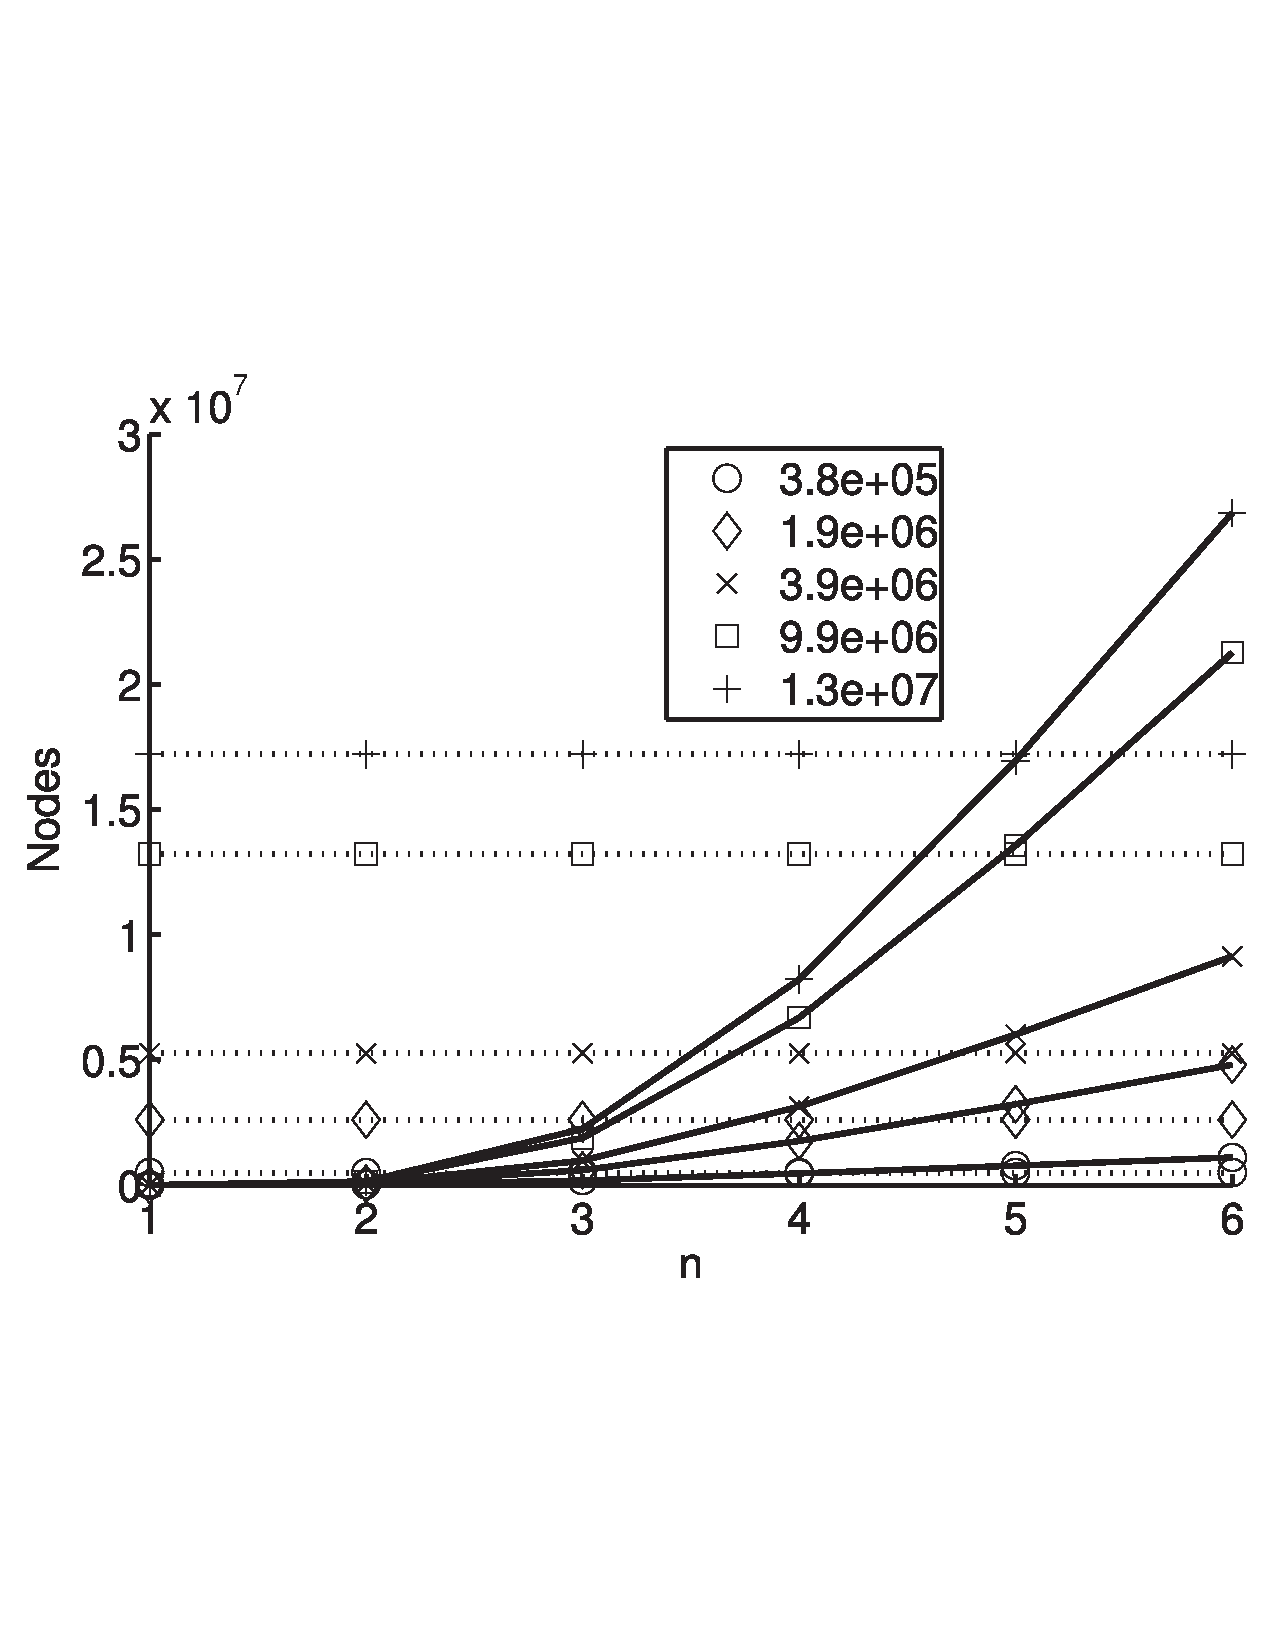
\includegraphics[trim = 0mm 60mm 00mm 60mm, clip, width=.4\textwidth]{fig1b.pdf}
\label{fig1a}
}
\hspace{1.5cm}
\subfigure[]{
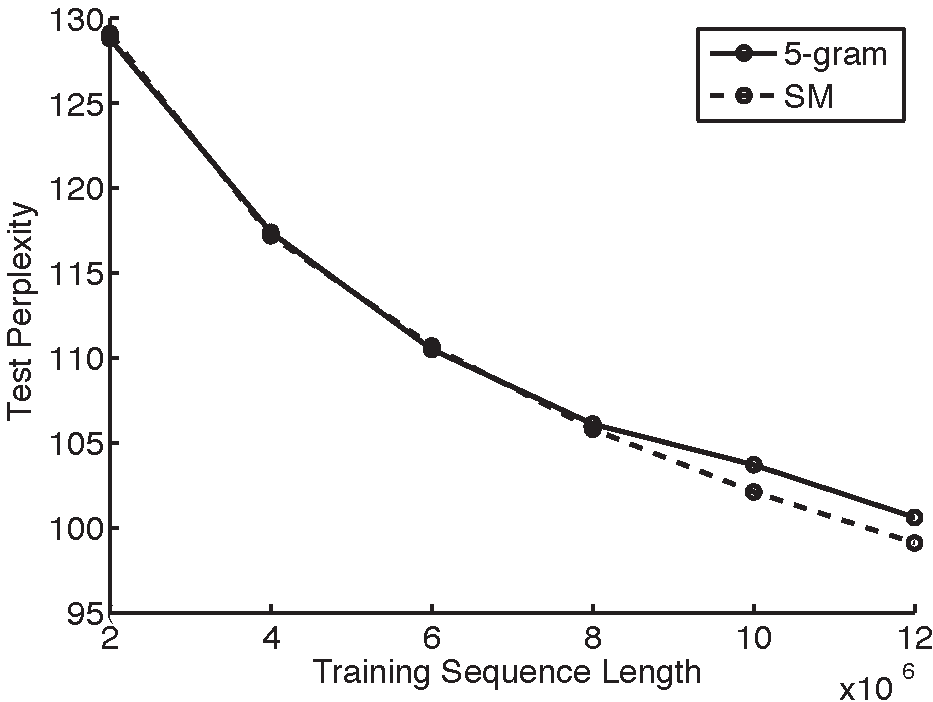
\includegraphics[width=.4\textwidth]{fig1.pdf}
\label{fig1b}
}
\caption{(a)  Memory complexity and estimation computational cost (in units of graphical model ``nodes'') versus $n$ of $n$-gram for the SM and a smoothing $n$-gram model.  There is one pair of lines for each of 5 different observation sequence lengths.  The horizontal dotted lines are the SM computational requirements.  The quadratic solid lines are the computational requirements the  smoothing $n$-gram models.  The SM always uses all contextual information when performing predictive inference.  The $n$-gram model discards contextual observations more distant than $n-1$.  None-the-less (a) shows that the computational complexity of each standard $n$-gram model exceeds that of a sequence memoizer trained on the same data for all $n>5$ and for all training observation sequence lengths.  This suggests that the sequence memoizer should be considered as an alternative to $n$-gram language modeling if long-range contextual dependencies matter.  The data used in this experiment was an excerpt of the New York times corpus.  (b)  Held-out test perplexity for two language models trained on growing excerpts of the Associated Press news corpus.  5-gram is a hierarchical Pitman-Yor process language model (a generalization of a Kneser Ney smoothed 5-gram model).  SM is the sequence memoizer.  Training sequence length ranges from 2-12 million tokens which we believe to be too small to characterize the benefit of being able to model and use long range dependencies.  Regardless, (b) suggests that held-out perplexity under the SM seems to improve relative to the smoothed $n$-gram model as more data is introduced into the model.  We conjecture that this is due to increasing prevalence of meaningful long contexts.  Experiments such as those proposed herein on larger corpora would establish the veracity of this conjecture.  Both of these figures were taken from \cite{Wood2009}.}
\label{default}
\end{center}
\end{figure}

We have already begun to demonstrate the practical utility of the SM, and in particular the benefits it extends beyond fixed, finite-depth $n$-gram models.  Various studies have found evidence of improvements to natural language models for automated speech recognition and machine translation, better encoding models for lossless compressors, and so forth.  These benefits seem to accrue from by being able to model and use the extra information that longer contexts provide, but much more experimentation is required to verify this observation.  We feel that an important scientific question remains unanswered: what happens to the importance of long-range contextual information as the amount of training data is increased?  Our intuition suggests that long-range dependencies will become more valuable, and the advantage of the SM relative to $n$-gram language models will grow, but currently the answer to this question remains unknown.   Further, the software and hardware infrastructure needed to answer this question do not currently exist.  One of the main purposes of this proposal is to start to address this question.

We have taken several theoretical and practical steps beyond the initial version of the SM; incremental estimation of the SM and the coupling of it to an entropy coder resulted in a highly competitive general purpose lossless compressor (significantly better than, for instance, gzip and bzip2) that scaled sufficiently to encode and compress a 100MB wikipedia corpus (1.6 bits / byte) \citep{Gasthaus2010}.  Following on that work, we have taken steps towards the development of a constant space, linear time approach to estimation of a class of models that includes the SM  \citep{Bartlett2010}.  This work  opens up for the first the possibility of performing experiments on large scale sequence data including the tera-word Google corpus.   No one knows what will happen when a powerful NPB language model such as the SM is trained on orders of magnitude more data than ever before.  Most of the engineering work necessary to achieve the asymptotic complexity results established in \citep{Bartlett2010} (constant space storage, linear time estimation, constant time inference) remains to be done, but we know it can be.  This means that many of the most interesting questions about the value of long-range contextual dependencies and the inferential power of BNP language models finally have a chance to be answered.

%In the course of pursuing this line of research, several pressing questions have emerged, the answers to which both have significant practical and theoretical importance.  We propose to answer these questions over the course of this project.

\comment{
\vspace{.1cm}
\noindent{\bf \large Sequence Memoizer}
\vspace{.1cm}

The SM \citep{Wood2009} consists of a hierarchical Bayesian nonparametric \citep{Teh2006a} prior
composed of Pitman-Yor processes married to efficient methods for representing and doing Bayesian inference in the resulting model. 
\def\GG{\mathcal{G}} The sequence memoizer describes the conditional probability of each
symbol $s$ following each context $\ubf$ using a latent variable $G_\ubf(s).$  Each symbol $s$ is a member of a set of symbols $\Sigma$.  
Collecting the natural set of such variables into a vector, $G_\ubf=[G_\ubf(s)]_{s\in\Sigma}$ results in $G_\ubf$ being a
probability vector (non-negative entries summing to one).   There is one such distribution for every context $\ubf$.    The full
(infinite) set of latent variables in the model (all the nodes in an infinitely deep tree) is denoted by
$\GG=\{G_\ubf\}_{\ubf\in\Sigma^*}$.  




The joint\footnote{Recall that a joint distribution can always be factored into the product of conditional distributions of increasing context, i.e.~$P(x_1,\ldots,x_i|\theta) = P(x_1|\theta) P(x_2 | x_1, \theta) P(x_3 | x_1,x_2, \theta) \cdots P(x_i | \xbf_{1:(i-1)}, \theta)$} probability of $\xbf$ and $\GG$
is simply:
\begin{align}
P(\xbf,\GG) = P(\GG)\prod_{i=0}^{|\xbf|-1}G_{\xbf_{1:i}}(\xbf_{i+1})
\end{align}
where the rightmost term is the probability of each symbol conditioned on the sequence thus far, and $P(\GG)$ is the prior over the variables.  Bayesian inference is possible in this model and means that one can integrate out $\GG$ (by sequential importance sampling and Monte Carlo integration for instance), to get a marginal joint distribution $P(\xbf)$ over the sequence from which the various predictive distributions of interest can straightforwardly be derived.  
%Section \ref{sec:inference} describes how the algorithm in Section \ref{algorithm} is an approximation of this ideal Bayesian approach.

The prior used in the SM over the infinite set $\GG=\{G_\ubf\}_{\ubf\in\Sigma^*}$ of probability vectors is based on a hierarchical Bayesian model consisting of Pitman Yor processes.
\comment{\footnote{
In this paper we exclusively refer to a simplified Pitman-Yor process.  The Pitman-Yor process (PYP) \citep{Pitman1997}, denoted $\py(d,H)$, is a
distribution over probability vectors.   
It is parameterized by a \emph{discount parameter} $d \in (0,1)$ and a
probability vector $H$ called the \emph{base vector}.  If $G\sim\py(d,H)$ is a
Pitman-Yor distributed random probability vector, then the base vector is
simply its mean $\text{E}[G(s)]=H(s)$ while the discount parameter is related
to its variance $\text{Var}[G(s)]=(1-d)H(s)(1-H(s))$, for each $s\in\Sigma$.}}
%
%The sequence memoizer \citep{wood2009sms} is an extension of the general HPYP
%model described above to context of unbounded length, i.e. $\ubf$ is not
%restricted to maximum length, leading to a context tree of unbounded depth. 
%In order to make inference in such a model feasible through marginalization
%(described in the next paragraph), the parameter space of
%the PYP has to be restricted to $\alpha=0$. 
Succinctly, we can notate the SM prior as follows:
\begin{subequations}
        \label{eqn:sm_prior}
        \begin{align}
            G_{\varepsilon} \mid d_0,H\quad &\sim \quad\py(d_0,H) \label{eq:m1} &\\
            G_{\ubf} \mid d_{|\ubf|},G_{\suffix(\ubf)} \quad
            &\sim \quad \py(d_{|\ubf|},G_{\suffix(\ubf)})  & \forall \ubf \in
            \Sigma^+ \label{eq:m2}\\
            x_i \mid \xbf_{1:i-1}=\ubf \quad &\sim\quad  G_{[\ubf]} 
            &  
            i=1,\ldots,T \label{eq:m3}
        \end{align}
\end{subequations}
\noindent where $H$ is a base probability distribution vector (in the following assumed to be
uniform over a finite vocabulary) and $d_{|\ubf|}$ are PYP parameters.
%The SM model is a hierarchical prior placed on the set of distributions
%$\{G_{[\ubf]}\}_{\ubf \in \Sigma^{*}}$, where $G_{[\ubf]}(v)$  corresponds
%to the probability of symbol $v \in \Sigma$ following the context $\ubf$.
%The structure of the model is an unbounded-depth tree, with each node indexed by a context $\ubf\in\Sigma^*$, labelled by the probability vector $G_\ubf$, and with parent given by $\sigma(\ubf)$.   %A binary sequence memoizer model is shown in Fig.~\ref{fig: gm_binary_complete}.
}
\comment{
\section{Expected Outcomes and Results}

\begin{itemize}
\item A scalable implementation of the sequence memoizer that researchers in the community can download and use in their own work.  (a webpage and link to sequence memoizer source code and/or library)
\item A publication relating implementation details and baseline perplexity (language modeling) and log loss (compression) results for sequence memoizers trained using Google-scale data 
\item latent variable extension (combining the sequence memoizer with, for instance, the infinite hierarchical Markov model \citep{Heller2009} or latent Dirichlet allocation \citep{Blei2003}, and develop scalable incremental estimation procedures for the combination.
\end{itemize}
}
\vspace{.1cm}
}%
\vspace{.1cm}
\noindent{\bf Annual Budget}
\vspace{.1cm}% budget.tex
% defs for below.  note " " after defs.
\def\piA{Person A }
\def\piB{Person B }
\def\numRAs{2 }
\def\pilist{PIs: \piA and \piB}
\def\thisyear{2006}
\def\startdate{06/01/2007 }
\def\enddate{05/31/2010 }
\def\phdstipend{\$2,125/mo }
\def\mscstipend{\$1,940/mo }
\def\studraise{4\% }
\def\salaryallocationrate{8.34\%} % no trailing space
\def\employeebenefitrate{27.0\% }
\def\vacationaccrualrate{9.5\% }
\def\networkservicescost{\$100/person/month }
\def\networkfacilitycharges{\$150/person/month} % no trailing space
\def\MITninemonthtuition{\$33,400} % no trailing space
\def\MITtuitioninflator{4\% }
\def\MITtuitionsubsidy{45\% }
\def\MITtuitioncharge{55\% }
\def\msAllocation{1.24\%}
\def\facostinception{07/01/2006} % no trailing space
\def\facostrate{65\% }

% make the outer enumerated list alpha A, B, C ...
\renewcommand{\theenumi}{\Alph{enumi}}
\renewcommand{\theenumii}{\arabic{enumii}}

\vspace*{1.0in}
\begin{center}
{\large
MIT / Computer Science and Artificial Intelligence Laboratory \\
\pilist \\
Proposed Budget Period: \startdate -- \enddate \\
Budget Justification for Cost Proposal
}
\end{center}

\begin{enumerate}

%A
\item \underline{Key Personnel:}

\begin{tabular}{|l|l|} \hline
\underline{Last Name} & \underline{Review/Raise} \\ \hline
\piA & June \\ \hline
\piB & June \\ \hline
\end{tabular}

MIT fully supports the academic year salaries of professors, associate
professors, and assistant professors, but makes no specific commitment
of time or salary to any individual research project.

%B
\item \underline{Other Personnel:}

\begin{enumerate}
  \item \underline{Research Assistants:} \\{~}\\
100\% of the stipend is charged to the research project. The RA stipend
is not subject to employee benefits. Stipend for the year beginning on
\startdate is \phdstipend for a PhD student and \mscstipend for a
Masters student. A \studraise raise is applied each year (in June).

%2
  \item \underline{Other (Technical \& Administrative Support):}\\{~}\\
The Computer Science Artificial Intelligence Laboratory (CSAIL) provides administrative
services for all principal investigators who submit proposals through CSAIL. These
administrative services are run by the Headquarters Staff and include Fiscal, Personnel,
Facilities and other CSAIL operations.\\{~}\\
These services are supported by an Allocated Project Level Cost, which is assessed against all
contracts and grants. The current rate for the Salary Allocation is \salaryallocationrate. The Allocation
Base is shown below:

\begin{tabular}{|c|c|c|c|} \hline
Allocation & Year 1 & Year 2 & Year 3 \\ \hline
Base & \$XXX,YYY & \$XXX,YYY & \$XXX,YYY \\ \hline
\end{tabular}

\end{enumerate}

\item \underline{Fringe Benefits}

\begin{enumerate}

%(a)
\item Employee benefits are calculated at the rate of \employeebenefitrate and 
are applied to total salary expenses, less Research Assistants.

\item Vacation accruals are calculated at the rate of \vacationaccrualrate and 
are applied to total salary expenses, less Faculty and Research
Assistants.

\end{enumerate}

%D
\item \underline{Travel:}

\begin{enumerate}

\item \underline{Domestic Travel:}

\item \underline{Foreign Travel:}

\end{enumerate}

\item \underline{Other Direct Costs:}

\begin{enumerate}

\item \underline{Material \& Supplies:}\\{~}\\
Estimated costs for software and supplies needed for the project.

\item \underline{Computer Services:}\\{~}\\
MIT/CSAIL has a centralized network services function. The costs consist of Network Services at
\networkservicescost and Network Facility Charges at \networkfacilitycharges. The base number of
people used for this calculation was \numRAs (the two full time RAs).

\item \underline{Other:}\\{~}\\
(a) RA tuition: For the academic year starting \thisyear, MIT 9-month
tuition is \MITninemonthtuition. A \MITtuitioninflator annual inflator
is applied each year. MIT will subsidize \MITtuitionsubsidy of tuition,
leaving \MITtuitioncharge to be charged to the project. During the
summer, MIT has waived tuition.\\{~}\\ 
(b) Allocated expenses are assessed against all contracts and
grants. The current rate for the Materials and Services Allocation is
\msAllocation. These funds help support the Headquarters staff mentioned
above in the section entitled ``Other (Technical \& Administrative
Support)''. Please see the table in that section for the allocation
base.

\item \underline{Equipment:}

The equipment line items will support purchases as follows:

\begin{itemize}

\item Year One (\$X,XXX): enter purpose, items and costs here

\item Year Two (\$X,XXX): enter purpose, items and costs here

\item Year Three (\$X,XXX): enter purpose, items and costs here

\end{itemize}

\item \underline{[Describe any other direct cost items here]:}

\end{enumerate}

\item \underline{Indirect Costs (Facilities \& Administrative Costs):}\\{~}\\
Effective \facostinception, F\&A Costs are calculated by applying the
negotiated rate of \facostrate to the Modified Total Direct Cost (MTDC)
base. The MTDC base includes all direct costs, except Graduate Student
Tuition, Network Facilities Charges, the Salary Allocation (and
associated benefits), and the Materials and Services Allocation.

\end{enumerate}


%\subsection{}
\newpage
%\section{References}
\small
\bibliography{../../../papers/uber.bib}
\bibliographystyle{apalike}

\end{document}  